% !TeX program = xelatex
\documentclass{article}
\usepackage{kotex}
\usepackage[a4paper,left=3cm, right=3cm, top=2cm, bottom=2cm]{geometry}
\usepackage{amsmath}
\usepackage{graphicx}
\usepackage{caption}
\usepackage{setspace}
\usepackage{xcolor}
\usepackage{titlesec}
\usepackage{amssymb}
\usepackage{tcolorbox}
\usepackage{wrapfig}
\usepackage{amsthm}
\usepackage{multirow}
\usepackage{array}
\usepackage{tikz}
\usepackage{longtable}
\usepackage{pgfplots}
\pgfplotsset{compat=1.18}

\title{1.7 Diagonal, Triangular, and Symmetric Matrices}
\date{}
\author{}
\setstretch{1.3}

\titleformat{name=\section, numberless}
  {\normalfont\large\bfseries\color{blue}}
  {}
  {0pt}
  {}
\geometry{a4paper, margin=1in}

\newcommand{\redheading}[1]{{\vspace{2mm}\noindent\Large\bfseries\color{red!55!black} #1\par}\vspace{2mm}}

\newtheoremstyle{mystyle}
  {}{}{\itshape}{}{\bfseries}{.}{.5em}{}
\theoremstyle{mystyle}

\begin{document}
\maketitle

{\itshape\color{blue!45!black}
This section discusses matrices with special forms---diagonal, triangular, and symmetric---that arise in a wide variety of applications and play an important role in subsequent work.\par}

\redheading{Diagonal Matrices}

A square matrix with all off-diagonal entries equal to zero is called a \textbf{diagonal matrix}. Examples:
\[
\begin{bmatrix}2&0\\0&-5\end{bmatrix},\quad
\begin{bmatrix}1&0&0\\0&1&0\\0&0&1\end{bmatrix},\quad
\begin{bmatrix}6&0&0&0\\0&-4&0&0\\0&0&0&0\\0&0&0&8\end{bmatrix},\quad
\begin{bmatrix}0&0\\0&0\end{bmatrix}
\]
A general $n\times n$ diagonal matrix $D$ has the form
\begin{equation}
D=\begin{bmatrix}d_1&0&\cdots&0\\0&d_2&\cdots&0\\\vdots&\vdots&&\vdots\\0&0&\cdots&d_n\end{bmatrix} \tag{1}
\end{equation}
$D$ is invertible iff all diagonal entries are nonzero, in which case
\begin{equation}
D^{-1}=\begin{bmatrix}1/d_1&0&\cdots&0\\0&1/d_2&\cdots&0\\\vdots&\vdots&&\vdots\\0&0&\cdots&1/d_n\end{bmatrix} \tag{2}
\end{equation}
For a positive integer $k$, powers of $D$ are also diagonal:
\begin{equation}
D^k=\begin{bmatrix}d_1^k&0&\cdots&0\\0&d_2^k&\cdots&0\\\vdots&\vdots&&\vdots\\0&0&\cdots&d_n^k\end{bmatrix} \tag{3}
\end{equation}

\subsection*{EXAMPLE 1 | Inverses and Powers of Diagonal Matrices}
For $A=\begin{bmatrix}1&0&0\\0&-3&0\\0&0&2\end{bmatrix}$, formulas (2) and (3) give
\[
A^{-1}=\begin{bmatrix}1&0&0\\0&-\frac{1}{3}&0\\0&0&\frac{1}{2}\end{bmatrix},\qquad
A^5=\begin{bmatrix}1&0&0\\0&-243&0\\0&0&32\end{bmatrix},\qquad
A^{-5}=\begin{bmatrix}1&0&0\\0&-\frac{1}{243}&0\\0&0&\frac{1}{32}\end{bmatrix}
\]

Products involving diagonal factors are especially easy to compute. Multiplying a matrix $A$ \emph{on the left} by diagonal $D$ scales successive \emph{rows} of $A$ by $d_1,d_2,\ldots,d_n$; multiplying $A$ \emph{on the right} by $D$ scales successive \emph{columns} of $A$ by $d_1,d_2,\ldots,d_n$. For example:
\[
\begin{bmatrix}d_1&0&0\\0&d_2&0\\0&0&d_3\end{bmatrix}
\begin{bmatrix}a_{11}&a_{12}&a_{13}&a_{14}\\a_{21}&a_{22}&a_{23}&a_{24}\\a_{31}&a_{32}&a_{33}&a_{34}\end{bmatrix}
=
\begin{bmatrix}d_1a_{11}&d_1a_{12}&d_1a_{13}&d_1a_{14}\\d_2a_{21}&d_2a_{22}&d_2a_{23}&d_2a_{24}\\d_3a_{31}&d_3a_{32}&d_3a_{33}&d_3a_{34}\end{bmatrix}
\]

\redheading{Triangular Matrices}

A square matrix with all entries \emph{above} the main diagonal equal to zero is called \textbf{lower triangular}; one with all entries \emph{below} the main diagonal equal to zero is called \textbf{upper triangular}. A matrix that is either is called \textbf{triangular}.

\subsection*{EXAMPLE 2 | Upper and Lower Triangular Matrices}

\begin{center}
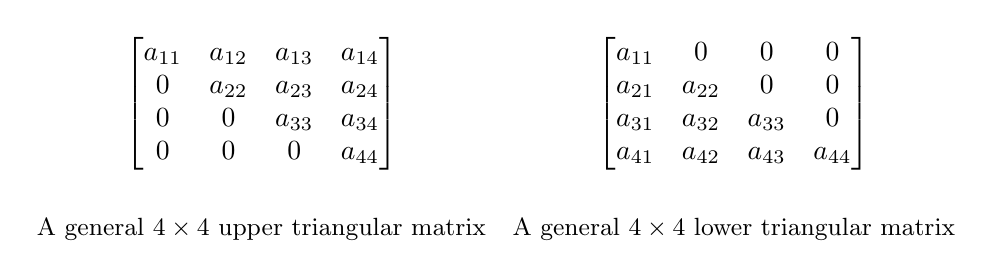
\begin{tikzpicture}
\node at (0,0) {$\begin{bmatrix}a_{11}&a_{12}&a_{13}&a_{14}\\0&a_{22}&a_{23}&a_{24}\\0&0&a_{33}&a_{34}\\0&0&0&a_{44}\end{bmatrix}$};
\node at (0,-1.6) {\small A general $4\times4$ upper triangular matrix};
\node at (6,0) {$\begin{bmatrix}a_{11}&0&0&0\\a_{21}&a_{22}&0&0\\a_{31}&a_{32}&a_{33}&0\\a_{41}&a_{42}&a_{43}&a_{44}\end{bmatrix}$};
\node at (6,-1.6) {\small A general $4\times4$ lower triangular matrix};
\end{tikzpicture}
\end{center}

\vspace{2mm}
\noindent\textbf{Remark.} Diagonal matrices are both upper and lower triangular. A square matrix in row echelon form is upper triangular.

The four basic properties of triangular matrices:
\begin{itemize}\setlength\itemsep{0pt}
  \item $A=[a_{ij}]$ is upper triangular iff $a_{ij}=0$ for $i>j$.
  \item $A=[a_{ij}]$ is lower triangular iff $a_{ij}=0$ for $i<j$.
  \item Upper triangular: the $i$th row starts with at least $i-1$ zeros for every $i$.
  \item Lower triangular: the $j$th column starts with at least $j-1$ zeros for every $j$.
\end{itemize}

\begin{tcolorbox}[colback=red!4, colframe=red!60!black, title=Theorem 1.7.1, boxrule=0.5mm, arc=3mm]
(a) The transpose of a lower triangular matrix is upper triangular, and vice versa.\\
(b) The product of lower triangular matrices is lower triangular, and the product of upper triangular matrices is upper triangular.\\
(c) A triangular matrix is invertible iff all its diagonal entries are nonzero.\\
(d) The inverse of an invertible lower triangular matrix is lower triangular, and the inverse of an invertible upper triangular matrix is upper triangular.
\end{tcolorbox}

\textbf{Proof (b)} We prove it for lower triangular; the upper triangular case is similar. Let $A=[a_{ij}]$ and $B=[b_{ij}]$ be lower triangular $n\times n$, and let $C=[c_{ij}]=AB$. We show $c_{ij}=0$ when $i<j$. From the definition of matrix multiplication,
\[
c_{ij}=a_{i1}b_{1j}+a_{i2}b_{2j}+\cdots+a_{in}b_{nj}
\]
For $i<j$, group the terms as
\[
c_{ij}=\underbrace{a_{i1}b_{1j}+\cdots+a_{i(j-1)}b_{(j-1)j}}_{\text{$b$ row index $<j$, so $B$ lower tri } \Rightarrow b_{kj}=0}+\underbrace{a_{ij}b_{jj}+\cdots+a_{in}b_{nj}}_{\text{$a$ row $i<$ col index, so $A$ lower tri }\Rightarrow a_{ik}=0}=0 \qquad\blacksquare
\]

\subsection*{EXAMPLE 3 | Computations with Triangular Matrices}
For upper triangular $A=\begin{bmatrix}1&3&-1\\0&2&4\\0&0&5\end{bmatrix}$ and $B=\begin{bmatrix}3&-2&2\\0&0&-1\\0&0&1\end{bmatrix}$:

By Theorem 1.7.1(c), $A$ is invertible (all diagonal entries nonzero) but $B$ is not ($b_{22}=0$). By parts (b) and (d), $A^{-1}$, $AB$, and $BA$ are all upper triangular:
\[
A^{-1}=\begin{bmatrix}1&-\frac{3}{2}&\frac{7}{5}\\0&\frac{1}{2}&-\frac{2}{5}\\0&0&\frac{1}{5}\end{bmatrix},\quad
AB=\begin{bmatrix}3&-2&-2\\0&0&2\\0&0&5\end{bmatrix},\quad
BA=\begin{bmatrix}3&5&-1\\0&0&-5\\0&0&5\end{bmatrix}
\]

\redheading{Symmetric Matrices}

\begin{tcolorbox}[colback=teal!4, colframe=teal!65!black, title=Definition 1, fonttitle=\bfseries, boxrule=0.5mm, arc=3mm]
A square matrix $A$ is \textbf{symmetric} if $A=A^T$.
\end{tcolorbox}

\subsection*{EXAMPLE 4 | Symmetric Matrices}
The following are symmetric (each equals its own transpose):
\[
\begin{bmatrix}7&-3\\-3&5\end{bmatrix},\quad
\begin{bmatrix}1&4&5\\4&-3&0\\5&0&7\end{bmatrix},\quad
\begin{bmatrix}d_1&0&0&0\\0&d_2&0&0\\0&0&d_3&0\\0&0&0&d_4\end{bmatrix}
\]

\textbf{Remark.} By Formula (14) of Section 1.3, $A=[a_{ij}]$ is symmetric iff
\begin{equation}
(A)_{ij}=(A)_{ji} \quad\text{for all }i,j \tag{4}
\end{equation}
Thus a symmetric matrix is characterized by the mirror symmetry of its entries about the main diagonal.

\begin{tcolorbox}[colback=red!4, colframe=red!60!black, title=Theorem 1.7.2, boxrule=0.5mm, arc=3mm]
If $A$ and $B$ are symmetric matrices of the same size, and $k$ is any scalar, then:\\
(a) $A^T$ is symmetric.\quad (b) $A+B$ and $A-B$ are symmetric.\quad (c) $kA$ is symmetric.
\end{tcolorbox}

The product of two symmetric matrices need not be symmetric. Indeed, if $A=A^T$ and $B=B^T$, then $(AB)^T=B^TA^T=BA$, so $AB$ is symmetric iff $AB=BA$:

\begin{tcolorbox}[colback=red!4, colframe=red!60!black, title=Theorem 1.7.3, boxrule=0.5mm, arc=3mm]
The product of two symmetric matrices is symmetric if and only if the matrices commute.
\end{tcolorbox}

\subsection*{EXAMPLE 5 | Products of Symmetric Matrices}
The first product below is \emph{not} symmetric (the factors do not commute); the second \emph{is} (the factors commute):
\[
\begin{bmatrix}1&2\\2&3\end{bmatrix}\begin{bmatrix}-4&1\\1&0\end{bmatrix}=\begin{bmatrix}-2&1\\-5&2\end{bmatrix},\qquad
\begin{bmatrix}1&2\\2&3\end{bmatrix}\begin{bmatrix}-4&3\\3&-1\end{bmatrix}=\begin{bmatrix}2&1\\1&3\end{bmatrix}
\]

\redheading{Invertibility of Symmetric Matrices}

A symmetric matrix need not be invertible (e.g.\ a diagonal matrix with a zero diagonal entry). However:

\begin{tcolorbox}[colback=red!4, colframe=red!60!black, title=Theorem 1.7.4, boxrule=0.5mm, arc=3mm]
If $A$ is an invertible symmetric matrix, then $A^{-1}$ is symmetric.
\end{tcolorbox}
\textbf{Proof} Since $A=A^T$, by Theorem 1.4.9 $(A^{-1})^T=(A^T)^{-1}=A^{-1}$, so $A^{-1}$ is symmetric. $\blacksquare$

\begin{tcolorbox}[colback=red!4, colframe=red!60!black, title=Theorem 1.7.5, boxrule=0.5mm, arc=3mm]
If $A$ is an invertible matrix, then $AA^T$ and $A^TA$ are also invertible.
\end{tcolorbox}
\textbf{Proof} Since $A$ is invertible, so is $A^T$ (Theorem 1.4.9). Hence $AA^T$ and $A^TA$ are products of invertible matrices and therefore invertible. $\blacksquare$

\redheading{Products $AA^T$ and $A^TA$ are Symmetric}

For any $m\times n$ matrix $A$, the products $AA^T$ (size $m\times m$) and $A^TA$ (size $n\times n$) are always defined and always symmetric:
\[
(AA^T)^T=(A^T)^TA^T=AA^T,\qquad (A^TA)^T=A^T(A^T)^T=A^TA
\]

\subsection*{EXAMPLE 6 | The Product of a Matrix and Its Transpose Is Symmetric}
For the $2\times3$ matrix $A=\begin{bmatrix}1&-2&4\\3&0&-5\end{bmatrix}$:
\[
A^TA=\begin{bmatrix}1&3\\-2&0\\4&-5\end{bmatrix}\begin{bmatrix}1&-2&4\\3&0&-5\end{bmatrix}=\begin{bmatrix}10&-2&-11\\-2&4&-8\\-11&-8&41\end{bmatrix}
\]
\[
AA^T=\begin{bmatrix}1&-2&4\\3&0&-5\end{bmatrix}\begin{bmatrix}1&3\\-2&0\\4&-5\end{bmatrix}=\begin{bmatrix}21&-17\\-17&34\end{bmatrix}
\]
Both $A^TA$ and $AA^T$ are symmetric, as expected.

\section*{Exercise Set 1.7}
\begin{enumerate}
    \item[1.] Classify each matrix as upper triangular, lower triangular, diagonal (note: a diagonal matrix is both), or none of these.\\[2pt]
    (a) $\begin{bmatrix}2&1\\0&3\end{bmatrix}$\quad
    (b) $\begin{bmatrix}0&0\\4&0\end{bmatrix}$\quad
    (c) $\begin{bmatrix}-1&0&0\\0&2&0\\0&0&\frac{1}{5}\end{bmatrix}$\quad
    (d) $\begin{bmatrix}3&-2&7\\0&0&3\\0&0&8\end{bmatrix}$

    \item[3.] Find the product by inspection (using the diagonal multiplication rule).
    \[
    \begin{bmatrix}3&0&0\\0&-1&0\\0&0&2\end{bmatrix}\begin{bmatrix}2&1\\-4&1\\2&5\end{bmatrix}
    \]

    \item[7.] Find $A^2$, $A^{-2}$, and $A^{-k}$ (where $k$ is any integer) by inspection.
    \[
    A=\begin{bmatrix}1&0\\0&-2\end{bmatrix}
    \]

    \item[8.] Find $A^2$, $A^{-2}$, and $A^{-k}$ by inspection.
    \[
    A=\begin{bmatrix}-6&0&0\\0&3&0\\0&0&5\end{bmatrix}
    \]

    \item[11.] Compute the product by inspection.
    \[
    \begin{bmatrix}1&0&0\\0&0&0\\0&0&3\end{bmatrix}
    \begin{bmatrix}2&0&0\\0&5&0\\0&0&0\end{bmatrix}
    \begin{bmatrix}0&0&0\\0&2&0\\0&0&1\end{bmatrix}
    \]

    \item[13.] Compute the indicated power by inspection.
    \[
    \begin{bmatrix}1&0\\0&-1\end{bmatrix}^{39}
    \]

    \item[15.] Use the diagonal multiplication rule to compute the product by inspection.
    \[
    \begin{bmatrix}a&0&0\\0&b&0\\0&0&c\end{bmatrix}
    \begin{bmatrix}u&v\\w&x\\y&z\end{bmatrix}
    \quad\text{and}\quad
    \begin{bmatrix}r&s&t\\u&v&w\\x&y&z\end{bmatrix}
    \begin{bmatrix}a&0&0\\0&b&0\\0&0&c\end{bmatrix}
    \]

    \item[17.] Create a symmetric matrix by substituting appropriate numbers for the $\times$'s.\\[2pt]
    (a) $\begin{bmatrix}2&-1\\\times&3\end{bmatrix}$\qquad
    (b) $\begin{bmatrix}1&\times&\times&\times\\3&1&\times&\times\\7&-8&0&\times\\2&-3&9&0\end{bmatrix}$

    \item[19.] Determine whether the matrix is invertible by inspection.
    \[
    \begin{bmatrix}0&6&-1\\0&7&-4\\0&0&-2\end{bmatrix}
    \]

    \item[21.] Determine whether the matrix is invertible by inspection.
    \[
    \begin{bmatrix}1&0&0&0\\2&-5&0&0\\4&-3&4&0\\1&-2&1&3\end{bmatrix}
    \]

    \item[23.] Find the diagonal entries of $AB$ by inspection.
    \[
    A=\begin{bmatrix}3&2&6\\0&1&-2\\0&0&-1\end{bmatrix},\quad
    B=\begin{bmatrix}-1&2&7\\0&5&3\\0&0&6\end{bmatrix}
    \]

    \item[25.] Find all values of $a$ (if any) for which $A$ is symmetric.
    \[
    A=\begin{bmatrix}4&-3\\a+5&-1\end{bmatrix}
    \]

    \item[26.] Find all values of $a$, $b$, $c$ for which $A$ is symmetric.
    \[
    A=\begin{bmatrix}2&a-2b+2c&2a+b+c\\3&5&a+c\\0&-2&7\end{bmatrix}
    \]

    \item[27.] Find all values of $x$ for which $A$ is invertible.
    \[
    A=\begin{bmatrix}x-1&x^2&x^4\\0&x+2&x^3\\0&0&x-4\end{bmatrix}
    \]

    \item[29.] If $A$ is an invertible upper triangular or lower triangular matrix, what can you say about the diagonal entries of $A^{-1}$?

    \item[30.] Show that if $A$ is a symmetric $n\times n$ matrix and $B$ is any $n\times m$ matrix, then the following products are symmetric: $B^TB$, $BB^T$, $B^TAB$.

    \item[31.] Find a diagonal matrix $A$ that satisfies $A^5=\begin{bmatrix}1&0&0\\0&-1&0\\0&0&-1\end{bmatrix}$.

    \item[33.] Verify Theorem 1.7.1(b) for the matrix product $AB$ and Theorem 1.7.1(d) for the matrix $A$, where
    \[
    A=\begin{bmatrix}-1&2&5\\0&1&3\\0&0&-4\end{bmatrix},\quad
    B=\begin{bmatrix}2&-8&0\\0&2&1\\0&0&3\end{bmatrix}
    \]

    \item[34.] Let $A$ be an $n\times n$ symmetric matrix.\\
    (a) Show that $A^2$ is symmetric.\\
    (b) Show that $2A^2-3A+I$ is symmetric.

    \item[37.] Let $A=[a_{ij}]$ be an $n\times n$ matrix. Determine whether $A$ is symmetric.\\
    (a) $a_{ij}=i^2+j^2$\quad (b) $a_{ij}=i^2-j^2$\quad (c) $a_{ij}=2i+2j$\quad (d) $a_{ij}=2i^2+2j^3$
\end{enumerate}

\end{document}
